\chapter{The Dappled Grays}

The baron, followed by the count, traversed a long series of
apartments, in which the prevailing characteristics were heavy
magnificence and the gaudiness of ostentatious wealth, until he reached
the boudoir of Madame Danglars—a small octagonal-shaped room, hung with
pink satin, covered with white Indian muslin. The chairs were of
ancient workmanship and materials; over the doors were painted sketches
of shepherds and shepherdesses, after the style and manner of Boucher;
and at each side pretty medallions in crayons, harmonizing well with
the furnishings of this charming apartment, the only one throughout the
great mansion in which any distinctive taste prevailed. The truth was,
it had been entirely overlooked in the plan arranged and followed out
by M. Danglars and his architect, who had been selected to aid the
baron in the great work of improvement solely because he was the most
fashionable and celebrated decorator of the day. The decorations of the
boudoir had then been left entirely to Madame Danglars and Lucien
Debray. M. Danglars, however, while possessing a great admiration for
the antique, as it was understood during the time of the Directory,
entertained the most sovereign contempt for the simple elegance of his
wife’s favorite sitting-room, where, by the way, he was never permitted
to intrude, unless, indeed, he excused his own appearance by ushering
in some more agreeable visitor than himself; and even then he had
rather the air and manner of a person who was himself introduced, than
that of being the presenter of another, his reception being cordial or
frigid, in proportion as the person who accompanied him chanced to
please or displease the baroness.

Madame Danglars (who, although past the first bloom of youth, was still
strikingly handsome) was now seated at the piano, a most elaborate
piece of cabinet and inlaid work, while Lucien Debray, standing before
a small work-table, was turning over the pages of an album.

Lucien had found time, preparatory to the count’s arrival, to relate
many particulars respecting him to Madame Danglars. It will be
remembered that Monte Cristo had made a lively impression on the minds
of all the party assembled at the breakfast given by Albert de Morcerf;
and although Debray was not in the habit of yielding to such feelings,
he had never been able to shake off the powerful influence excited in
his mind by the impressive look and manner of the count, consequently
the description given by Lucien to the baroness bore the highly-colored
tinge of his own heated imagination. Already excited by the wonderful
stories related of the count by de Morcerf, it is no wonder that Madame
Danglars eagerly listened to, and fully credited, all the additional
circumstances detailed by Debray. This posing at the piano and over the
album was only a little ruse adopted by way of precaution. A most
gracious welcome and unusual smile were bestowed on M. Danglars; the
count, in return for his gentlemanly bow, received a formal though
graceful courtesy, while Lucien exchanged with the count a sort of
distant recognition, and with Danglars a free and easy nod.

“Baroness,” said Danglars, “give me leave to present to you the Count
of Monte Cristo, who has been most warmly recommended to me by my
correspondents at Rome. I need but mention one fact to make all the
ladies in Paris court his notice, and that is, that he has come to take
up his abode in Paris for a year, during which brief period he proposes
to spend six millions of money. That means balls, dinners, and lawn
parties without end, in all of which I trust the count will remember
us, as he may depend upon it we shall him, in our own humble
entertainments.”

In spite of the gross flattery and coarseness of this address, Madame
Danglars could not forbear gazing with considerable interest on a man
capable of expending six millions in twelve months, and who had
selected Paris for the scene of his princely extravagance.

“And when did you arrive here?” inquired she.

“Yesterday morning, madame.”

“Coming, as usual, I presume, from the extreme end of the globe? Pardon
me—at least, such I have heard is your custom.”

“Nay, madame. This time I have merely come from Cadiz.”

“You have selected a most unfavorable moment for your first visit.
Paris is a horrible place in summer. Balls, parties, and \textit{fêtes} are
over; the Italian opera is in London; the French opera everywhere
except in Paris. As for the Théatre Français, you know, of course, that
it is nowhere. The only amusements left us are the indifferent races at
the Champ-de-Mars and Satory. Do you propose entering any horses at
either of these races, count?”

“I shall do whatever they do at Paris, madame, if I have the good
fortune to find someone who will initiate me into the prevalent ideas
of amusement.”

“Are you fond of horses, count?”

“I have passed a considerable part of my life in the East, madame, and
you are doubtless aware that the Orientals value only two things—the
fine breeding of their horses and the beauty of their women.”

“Nay, count,” said the baroness, “it would have been somewhat more
gallant to have placed the ladies first.”

“You see, madame, how rightly I spoke when I said I required a
preceptor to guide me in all my sayings and doings here.”

At this instant the favorite attendant of Madame Danglars entered the
boudoir; approaching her mistress, she spoke some words in an
undertone. Madame Danglars turned very pale, then exclaimed:

“I cannot believe it; the thing is impossible.”

“I assure you, madame,” replied the woman, “it is as I have said.”

Turning impatiently towards her husband, Madame Danglars demanded, “Is
this true?”

“Is what true, madame?” inquired Danglars, visibly agitated.

“What my maid tells me.”

“But what does she tell you?”

“That when my coachman was about to harness the horses to my carriage,
he discovered that they had been removed from the stables without his
knowledge. I desire to know what is the meaning of this?”

“Be kind enough, madame, to listen to me,” said Danglars.

“Oh, yes; I will listen, monsieur, for I am most curious to hear what
explanation you will give. These two gentlemen shall decide between us;
but, first, I will state the case to them. Gentlemen,” continued the
baroness, “among the ten horses in the stables of Baron Danglars, are
two that belong exclusively to me—a pair of the handsomest and most
spirited creatures to be found in Paris. But to you, at least, M.
Debray, I need not give a further description, because to you my
beautiful pair of dappled grays were well known. Well, I had promised
Madame de Villefort the loan of my carriage to drive tomorrow to the
Bois; but when my coachman goes to fetch the grays from the stables
they are gone—positively gone. No doubt M. Danglars has sacrificed them
to the selfish consideration of gaining some thousands of paltry
francs. Oh, what a detestable crew they are, these mercenary
speculators!”

“Madame,” replied Danglars, “the horses were not sufficiently quiet for
you; they were scarcely four years old, and they made me extremely
uneasy on your account.”

“Nonsense,” retorted the baroness; “you could not have entertained any
alarm on the subject, because you are perfectly well aware that I have
had for a month in my service the very best coachman in Paris. But,
perhaps, you have disposed of the coachman as well as the horses?”

“My dear love, pray do not say any more about them, and I promise you
another pair exactly like them in appearance, only more quiet and
steady.”

The baroness shrugged her shoulders with an air of ineffable contempt,
while her husband, affecting not to observe this unconjugal gesture,
turned towards Monte Cristo and said,—“Upon my word, count, I am quite
sorry not to have met you sooner. You are setting up an establishment,
of course?”

“Why, yes,” replied the count.

“I should have liked to have made you the offer of these horses. I have
almost given them away, as it is; but, as I before said, I was anxious
to get rid of them upon any terms. They were only fit for a young man.”

“I am much obliged by your kind intentions towards me,” said Monte
Cristo; “but this morning I purchased a very excellent pair of
carriage-horses, and I do not think they were dear. There they are.
Come, M. Debray, you are a connoisseur, I believe, let me have your
opinion upon them.”

As Debray walked towards the window, Danglars approached his wife.

“I could not tell you before others,” said he in a low tone, “the
reason of my parting with the horses; but a most enormous price was
offered me this morning for them. Some madman or fool, bent upon
ruining himself as fast as he can, actually sent his steward to me to
purchase them at any cost; and the fact is, I have gained 16,000 francs
by the sale of them. Come, don’t look so angry, and you shall have
4,000 francs of the money to do what you like with, and Eugénie shall
have 2,000. There, what do you think now of the affair? Wasn’t I right
to part with the horses?”

Madame Danglars surveyed her husband with a look of withering contempt.

“Great heavens?” suddenly exclaimed Debray.

“What is it?” asked the baroness.

“I cannot be mistaken; there are your horses! The very animals we were
speaking of, harnessed to the count’s carriage!”

“My dappled grays?” demanded the baroness, springing to the window.
“’Tis indeed they!” said she.

Danglars looked absolutely stupefied.

“How very singular,” cried Monte Cristo with well-feigned astonishment.

“I cannot believe it,” murmured the banker. Madame Danglars whispered a
few words in the ear of Debray, who approached Monte Cristo, saying,
“The baroness wishes to know what you paid her husband for the horses.”

“I scarcely know,” replied the count; “it was a little surprise
prepared for me by my steward, and cost me—well, somewhere about 30,000
francs.”

Debray conveyed the count’s reply to the baroness. Poor Danglars looked
so crest-fallen and discomfited that Monte Cristo assumed a pitying air
towards him.

“See,” said the count, “how very ungrateful women are. Your kind
attention, in providing for the safety of the baroness by disposing of
the horses, does not seem to have made the least impression on her. But
so it is; a woman will often, from mere wilfulness, prefer that which
is dangerous to that which is safe. Therefore, in my opinion, my dear
baron, the best and easiest way is to leave them to their fancies, and
allow them to act as they please, and then, if any mischief follows,
why, at least, they have no one to blame but themselves.”

Danglars made no reply; he was occupied in anticipations of the coming
scene between himself and the baroness, whose frowning brow, like that
of Olympic Jove, predicted a storm. Debray, who perceived the gathering
clouds, and felt no desire to witness the explosion of Madame Danglars’
rage, suddenly recollected an appointment, which compelled him to take
his leave; while Monte Cristo, unwilling by prolonging his stay to
destroy the advantages he hoped to obtain, made a farewell bow and
departed, leaving Danglars to endure the angry reproaches of his wife.

\begin{figure}[ht]
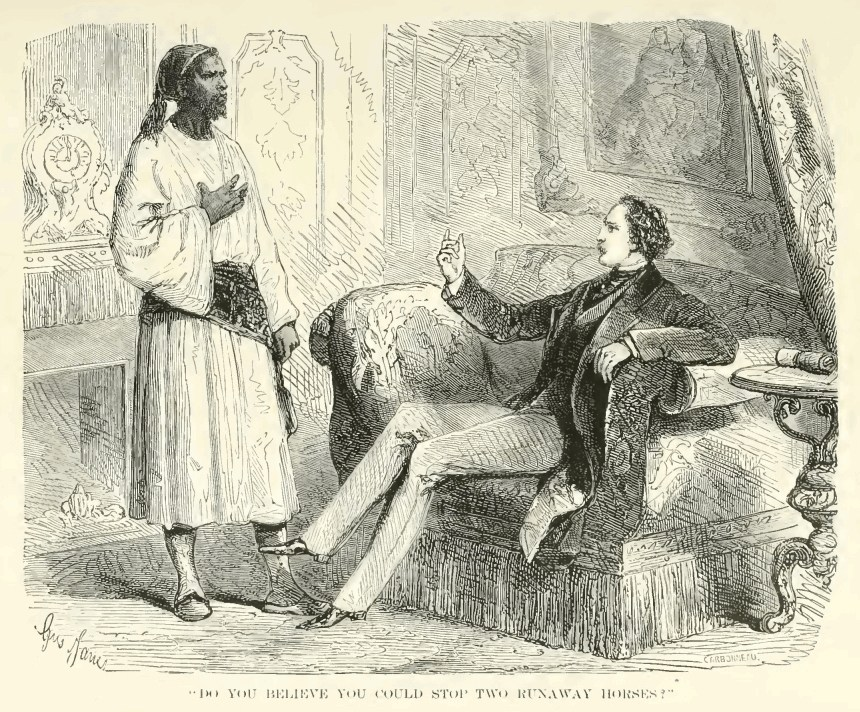
\includegraphics[width=\textwidth]{20347m.jpg}
\end{figure}

“Excellent,” murmured Monte Cristo to himself, as he came away. “All
has gone according to my wishes. The domestic peace of this family is
henceforth in my hands. Now, then, to play another master-stroke, by
which I shall gain the heart of both husband and wife—delightful!
Still,” added he, “amid all this, I have not yet been presented to
Mademoiselle Eugénie Danglars, whose acquaintance I should have been
glad to make. But,” he went on with his peculiar smile, “I am here in
Paris, and have plenty of time before me—by and by will do for that.”

With these reflections he entered his carriage and returned home. Two
hours afterwards, Madame Danglars received a most flattering epistle
from the count, in which he entreated her to receive back her favorite
“dappled grays,” protesting that he could not endure the idea of making
his entry into the Parisian world of fashion with the knowledge that
his splendid equipage had been obtained at the price of a lovely
woman’s regrets. The horses were sent back wearing the same harness she
had seen on them in the morning; only, by the count’s orders, in the
centre of each rosette that adorned either side of their heads, had
been fastened a large diamond.

To Danglars Monte Cristo also wrote, requesting him to excuse the
whimsical gift of a capricious millionaire, and to beg the baroness to
pardon the Eastern fashion adopted in the return of the horses.

During the evening, Monte Cristo quitted Paris for Auteuil, accompanied
by Ali. The following day, about three o’clock, a single blow struck on
the gong summoned Ali to the presence of the count.

“Ali,” observed his master, as the Nubian entered the chamber, “you
have frequently explained to me how more than commonly skilful you are
in throwing the lasso, have you not?”

Ali drew himself up proudly, and then returned a sign in the
affirmative.

“I thought I did not mistake. With your lasso you could stop an ox?”

Again Ali repeated his affirmative gesture.

“Or a tiger?”

Ali bowed his head in token of assent.

“A lion even?”

Ali sprung forwards, imitating the action of one throwing the lasso,
then of a strangled lion.

“I understand,” said Monte Cristo; “you wish to tell me you have hunted
the lion?”

Ali smiled with triumphant pride as he signified that he had indeed
both chased and captured many lions.

“But do you believe you could arrest the progress of two horses rushing
forwards with ungovernable fury?”

The Nubian smiled.

“It is well,” said Monte Cristo. “Then listen to me. Ere long a
carriage will dash past here, drawn by the pair of dappled gray horses
you saw me with yesterday; now, at the risk of your own life, you must
manage to stop those horses before my door.”

Ali descended to the street, and marked a straight line on the pavement
immediately at the entrance of the house, and then pointed out the line
he had traced to the count, who was watching him. The count patted him
gently on the shoulder, his usual mode of praising Ali, who, pleased
and gratified with the commission assigned him, walked calmly towards a
projecting stone forming the angle of the street and house, and,
seating himself thereon, began to smoke his chibouque, while Monte
Cristo re-entered his dwelling, perfectly assured of the success of his
plan.

Still, as five o’clock approached, and the carriage was momentarily
expected by the count, the indication of more than common impatience
and uneasiness might be observed in his manner. He stationed himself in
a room commanding a view of the street, pacing the chamber with
restless steps, stopping merely to listen from time to time for the
sound of approaching wheels, then to cast an anxious glance on Ali; but
the regularity with which the Nubian puffed forth the smoke of his
chibouque proved that he at least was wholly absorbed in the enjoyment
of his favorite occupation.

Suddenly a distant sound of rapidly advancing wheels was heard, and
almost immediately a carriage appeared, drawn by a pair of wild,
ungovernable horses, while the terrified coachman strove in vain to
restrain their furious speed.

In the vehicle was a young woman and a child of about seven or eight
clasped in each other’s arms. Terror seemed to have deprived them even
of the power of uttering a cry. The carriage creaked and rattled as it
flew over the rough stones, and the slightest obstacle under the wheels
would have caused disaster; but it kept on in the middle of the road,
and those who saw it pass uttered cries of terror.

Ali suddenly cast aside his chibouque, drew the lasso from his pocket,
threw it so skilfully as to catch the forelegs of the near horse in its
triple fold, and suffered himself to be dragged on for a few steps by
the violence of the shock, then the animal fell over on the pole, which
snapped, and therefore prevented the other horse from pursuing its way.
Gladly availing himself of this opportunity, the coachman leaped from
his box; but Ali had promptly seized the nostrils of the second horse,
and held them in his iron grasp, till the beast, snorting with pain,
sunk beside his companion.

All this was achieved in much less time than is occupied in the
recital. The brief space had, however, been sufficient for a man,
followed by a number of servants, to rush from the house before which
the accident had occurred, and, as the coachman opened the door of the
carriage, to take from it a lady who was convulsively grasping the
cushions with one hand, while with the other she pressed to her bosom
the young boy, who had lost consciousness. Monte Cristo carried them
both to the salon, and deposited them on a sofa.

“Compose yourself, madame,” said he; “all danger is over.” The woman
looked up at these words, and, with a glance far more expressive than
any entreaties could have been, pointed to her child, who still
continued insensible. “I understand the nature of your alarms, madame,”
said the count, carefully examining the child, “but I assure you there
is not the slightest occasion for uneasiness; your little charge has
not received the least injury; his insensibility is merely the effects
of terror, and will soon pass.”

“Are you quite sure you do not say so to tranquillize my fears? See how
deadly pale he is! My child, my darling Edward; speak to your
mother—open your dear eyes and look on me once again! Oh, sir, in pity
send for a physician; my whole fortune shall not be thought too much
for the recovery of my boy.”

With a calm smile and a gentle wave of the hand, Monte Cristo signed to
the distracted mother to lay aside her apprehensions; then, opening a
casket that stood near, he drew forth a phial of Bohemian glass
incrusted with gold, containing a liquid of the color of blood, of
which he let fall a single drop on the child’s lips. Scarcely had it
reached them, ere the boy, though still pale as marble, opened his
eyes, and eagerly gazed around him. At this, the delight of the mother
was almost frantic.

“Where am I?” exclaimed she; “and to whom am I indebted for so happy a
termination to my late dreadful alarm?”

“Madame,” answered the count, “you are under the roof of one who
esteems himself most fortunate in having been able to save you from a
further continuance of your sufferings.”

“My wretched curiosity has brought all this about,” pursued the lady.
“All Paris rung with the praises of Madame Danglars’ beautiful horses,
and I had the folly to desire to know whether they really merited the
high praise given to them.”

“Is it possible,” exclaimed the count with well-feigned astonishment,
“that these horses belong to the baroness?”

“They do, indeed. May I inquire if you are acquainted with Madame
Danglars?”

\begin{figure}[ht]
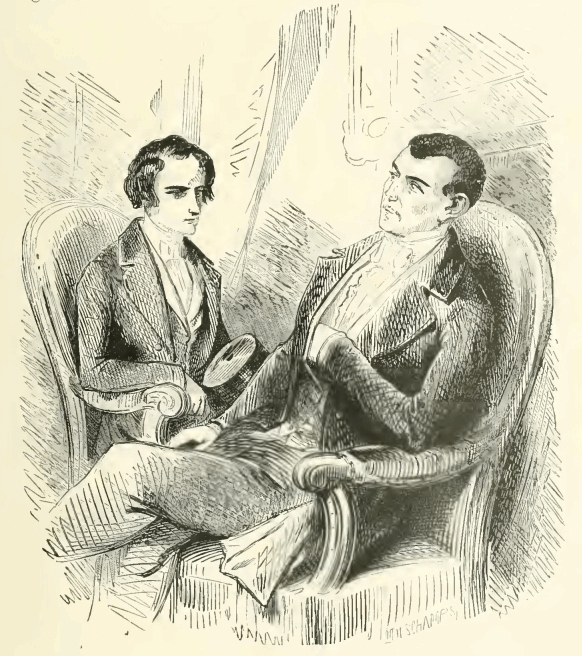
\includegraphics[width=\textwidth]{20351m.jpg}
\end{figure}

“I have that honor; and my happiness at your escape from the danger
that threatened you is redoubled by the consciousness that I have been
the unwilling and the unintentional cause of all the peril you have
incurred. I yesterday purchased these horses of the baron; but as the
baroness evidently regretted parting with them, I ventured to send them
back to her, with a request that she would gratify me by accepting them
from my hands.”

“You are, then, doubtless, the Count of Monte Cristo, of whom Hermine
has talked to me so much?”

“You have rightly guessed, madame,” replied the count.

“And I am Madame Héloïse de Villefort.”

The count bowed with the air of a person who hears a name for the first
time.

“How grateful will M. de Villefort be for all your goodness; how
thankfully will he acknowledge that to you alone he owes the existence
of his wife and child! Most certainly, but for the prompt assistance of
your intrepid servant, this dear child and myself must both have
perished.”

“Indeed, I still shudder at the fearful danger you were placed in.”

“I trust you will allow me to recompense worthily the devotion of your
man.”

“I beseech you, madame,” replied Monte Cristo “not to spoil Ali, either
by too great praise or rewards. I cannot allow him to acquire the habit
of expecting to be recompensed for every trifling service he may
render. Ali is my slave, and in saving your life he was but discharging
his duty to me.”

“Nay,” interposed Madame de Villefort, on whom the authoritative style
adopted by the count made a deep impression, “nay, but consider that to
preserve my life he has risked his own.”

“His life, madame, belongs not to him; it is mine, in return for my
having myself saved him from death.”

Madame de Villefort made no further reply; her mind was utterly
absorbed in the contemplation of the person who, from the first instant
she saw him, had made so powerful an impression on her.

During the evident preoccupation of Madame de Villefort, Monte Cristo
scrutinized the features and appearance of the boy she kept folded in
her arms, lavishing on him the most tender endearments. The child was
small for his age, and unnaturally pale. A mass of straight black hair,
defying all attempts to train or curl it, fell over his projecting
forehead, and hung down to his shoulders, giving increased vivacity to
eyes already sparkling with a youthful love of mischief and fondness
for every forbidden enjoyment. His mouth was large, and the lips, which
had not yet regained their color, were particularly thin; in fact, the
deep and crafty look, giving a predominant expression to the child’s
face, belonged rather to a boy of twelve or fourteen than to one so
young. His first movement was to free himself by a violent push from
the encircling arms of his mother, and to rush forward to the casket
from whence the count had taken the phial of elixir; then, without
asking permission of anyone, he proceeded, in all the wilfulness of a
spoiled child unaccustomed to restrain either whims or caprices, to
pull the corks out of all the bottles.

“Touch nothing, my little friend,” cried the count eagerly; “some of
those liquids are not only dangerous to taste, but even to inhale.”

Madame de Villefort became very pale, and, seizing her son’s arm, drew
him anxiously toward her; but, once satisfied of his safety, she also
cast a brief but expressive glance on the casket, which was not lost
upon the count. At this moment Ali entered. At sight of him Madame de
Villefort uttered an expression of pleasure, and, holding the child
still closer towards her, she said:

“Edward, dearest, do you see that good man? He has shown very great
courage and resolution, for he exposed his own life to stop the horses
that were running away with us, and would certainly have dashed the
carriage to pieces. Thank him, then, my child, in your very best
manner; for, had he not come to our aid, neither you nor I would have
been alive to speak our thanks.”

The child stuck out his lips and turned away his head in a disdainful
manner, saying, “He’s too ugly.”

\begin{figure}[ht]
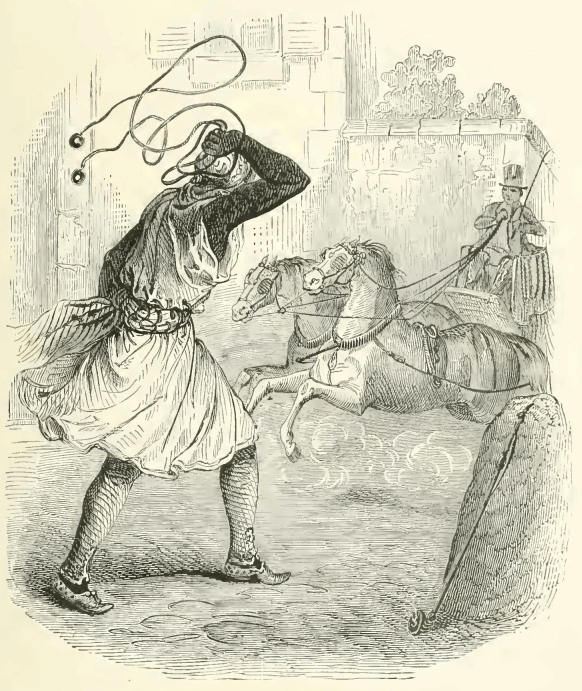
\includegraphics[width=\textwidth]{20353m.jpg}
\end{figure}

The count smiled as if the child bade fair to realize his hopes, while
Madame de Villefort reprimanded her son with a gentleness and
moderation very far from conveying the least idea of a fault having
been committed.

“This lady,” said the Count, speaking to Ali in the Arabic language,
“is desirous that her son should thank you for saving both their lives;
but the boy refuses, saying you are too ugly.”

Ali turned his intelligent countenance towards the boy, on whom he
gazed without any apparent emotion; but the spasmodic working of the
nostrils showed to the practiced eye of Monte Cristo that the Arab had
been wounded to the heart.

“Will you permit me to inquire,” said Madame de Villefort, as she arose
to take her leave, “whether you usually reside here?”

“No, I do not,” replied Monte Cristo; “it is a small place I have
purchased quite lately. My place of abode is No. 30, Avenue des
Champs-Élysées; but I see you have quite recovered from your fright,
and are, no doubt, desirous of returning home. Anticipating your
wishes, I have desired the same horses you came with to be put to one
of my carriages, and Ali, he whom you think so very ugly,” continued
he, addressing the boy with a smiling air, “will have the honor of
driving you home, while your coachman remains here to attend to the
necessary repairs of your calash. As soon as that important business is
concluded, I will have a pair of my own horses harnessed to convey it
direct to Madame Danglars.”

“I dare not return with those dreadful horses,” said Madame de
Villefort.

“You will see,” replied Monte Cristo, “that they will be as different
as possible in the hands of Ali. With him they will be gentle and
docile as lambs.”

Ali had, indeed, given proof of this; for, approaching the animals, who
had been got upon their legs with considerable difficulty, he rubbed
their foreheads and nostrils with a sponge soaked in aromatic vinegar,
and wiped off the sweat and foam that covered their mouths. Then,
commencing a loud whistling noise, he rubbed them well all over their
bodies for several minutes; then, undisturbed by the noisy crowd
collected round the broken carriage, Ali quietly harnessed the pacified
animals to the count’s chariot, took the reins in his hands, and
mounted the box, when to the utter astonishment of those who had
witnessed the ungovernable spirit and maddened speed of the same
horses, he was actually compelled to apply his whip in no very gentle
manner before he could induce them to start; and even then all that
could be obtained from the celebrated “dappled grays,” now changed into
a couple of dull, sluggish, stupid brutes, was a slow, pottering pace,
kept up with so much difficulty that Madame de Villefort was more than
two hours returning to her residence in the Faubourg Saint-Honoré.

\begin{figure}[ht]
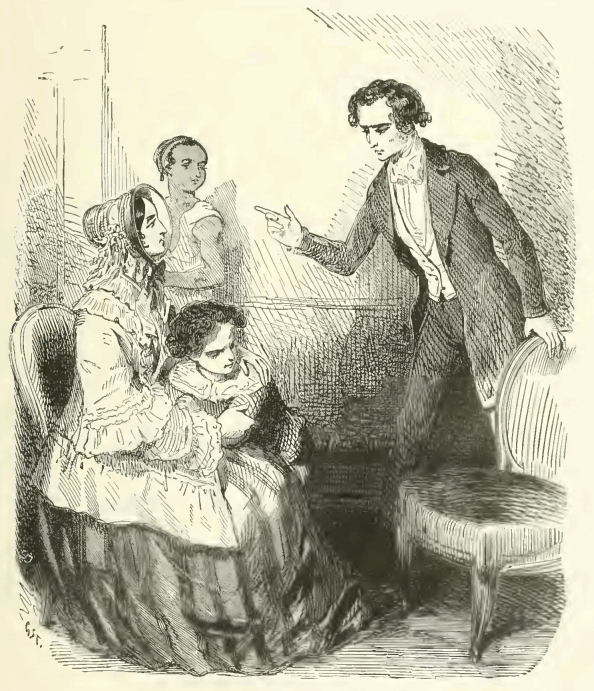
\includegraphics[width=\textwidth]{20355m.jpg}
\end{figure}

Scarcely had the first congratulations upon her marvellous escape been
gone through when she wrote the following letter to Madame Danglars:—

“Dear Hermine,—I have just had a wonderful escape from the most
imminent danger, and I owe my safety to the very Count of Monte Cristo
we were talking about yesterday, but whom I little expected to see
today. I remember how unmercifully I laughed at what I considered your
eulogistic and exaggerated praises of him; but I have now ample cause
to admit that your enthusiastic description of this wonderful man fell
far short of his merits. Your horses got as far as Ranelagh, when they
darted forward like mad things, and galloped away at so fearful a rate,
that there seemed no other prospect for myself and my poor Edward but
that of being dashed to pieces against the first object that impeded
their progress, when a strange-looking man,—an Arab, a negro, or a
Nubian, at least a black of some nation or other—at a signal from the
count, whose domestic he is, suddenly seized and stopped the infuriated
animals, even at the risk of being trampled to death himself; and
certainly he must have had a most wonderful escape. The count then
hastened to us, and took us into his house, where he speedily recalled
my poor Edward to life. He sent us home in his own carriage. Yours will
be returned to you tomorrow. You will find your horses in bad
condition, from the results of this accident; they seem thoroughly
stupefied, as if sulky and vexed at having been conquered by man. The
count, however, has commissioned me to assure you that two or three
days’ rest, with plenty of barley for their sole food during that time,
will bring them back to as fine, that is as terrifying, a condition as
they were in yesterday.

\begin{figure}[ht]
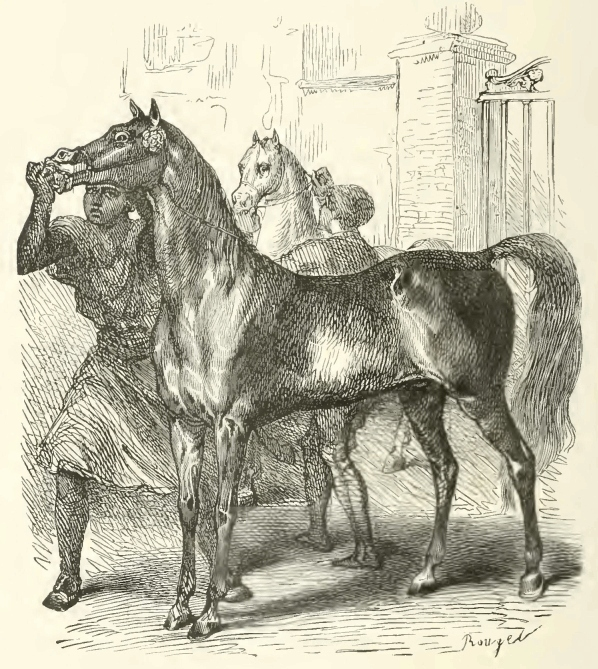
\includegraphics[width=\textwidth]{20356m.jpg}
\end{figure}

Adieu! I cannot return you many thanks for the drive of yesterday; but,
after all, I ought not to blame you for the misconduct of your horses,
more especially as it procured me the pleasure of an introduction to
the Count of Monte Cristo,—and certainly that illustrious personage,
apart from the millions he is said to be so very anxious to dispose of,
seemed to me one of those curiously interesting problems I, for one,
delight in solving at any risk, even if it were to necessitate another
drive to the Bois behind your horses.

Edward endured the accident with miraculous courage —he did not utter a
single cry, but fell lifeless into my arms; nor did a tear fall from
his eyes after it was over. I doubt not you will consider these praises
the result of blind maternal affection, but there is a soul of iron in
that delicate, fragile body. Valentine sends many affectionate
remembrances to your dear Eugénie. I embrace you with all my heart.

Héloïse de Villefort.

P.S.—Do pray contrive some means for me to meet the Count of Monte
Cristo at your house. I must and will see him again. I have just made
M. de Villefort promise to call on him, and I hope the visit will be
returned.

That night the adventure at Auteuil was talked of everywhere. Albert
related it to his mother; Château-Renaud recounted it at the Jockey
Club, and Debray detailed it at length in the salons of the minister;
even Beauchamp accorded twenty lines in his journal to the relation of
the count’s courage and gallantry, thereby celebrating him as the
greatest hero of the day in the eyes of all the feminine members of the
aristocracy.

Vast was the crowd of visitors and inquiring friends who left their
names at the residence of Madame de Villefort, with the design of
renewing their visit at the right moment, of hearing from her lips all
the interesting circumstances of this most romantic adventure.

As for M. de Villefort, he fulfilled the predictions of Héloïse to the
letter,—donned his dress suit, drew on a pair of white gloves, ordered
the servants to attend the carriage dressed in their full livery, and
drove that same night to No. 30 in the Avenue des Champs-Élysées.
